
\chapter{功能描述}

车载双向充电机(BOBC)功能要求;
主要参考资料:
\href{https://blog.csdn.net/hadywell/article/details/128699869?utm_medium=distribute.pc_relevant.none-task-blog-2~default~baidujs_utm_term~default-5-128699869-blog-112810903.235^v43^control&spm=1001.2101.3001.4242.4&utm_relevant_index=8}{新能源汽车充电硬件接口标准}

\begin{table}[h]
    \centering
    \caption{功能描述}
    \renewcommand{\arraystretch}{1.3}
    \begin{tabular}{|c|l|}
        \hline
        \cellcolor{yellow} 功能要求 & \cellcolor{yellow}功能描述\\
        \hline
        CC(Charging Connection)&充电连接确认:\\
        \hline
        CP(Control Pilot)&控制确认:\\
        \hline
    \end{tabular}
\end{table}


电动汽车的充电系统包括车载充电机、高压动力电池、电池管理系统、整
车控制器(Vehicle Control Unit, VCU)和充电桩五个部分。电动汽车进行充电时,
当充电枪插入电动汽车的充电接口后,并不是直接供给动力电池能量,而是先
检测来自充电桩的信号以判断最大可输入电流,然后完成与 BMS 和 VCU 完成
充电前的信息交互,最后进行充电,充电过程中,充电机始终保持与 BMS 和
VCU 的相互通信。
    \begin{figure}[!htbp]
        \centering
        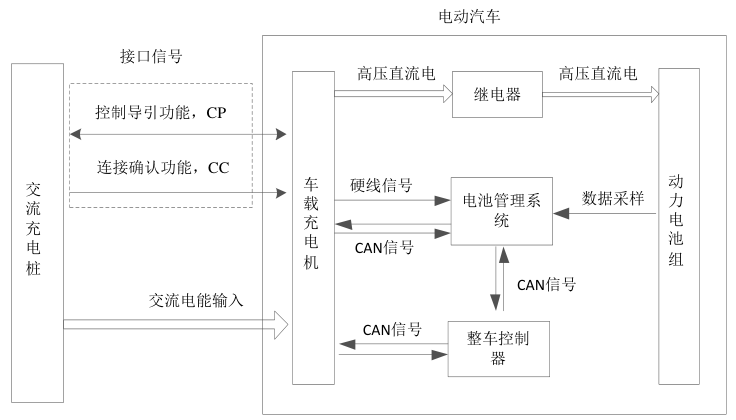
\includegraphics[width = 0.7\textwidth]{C1}
        \caption{电动汽车充电系统结构}
        \label{fig:C1}
    \end{figure}

如图\ref{fig:C1},根据 GB/T18487.1-2015\cite{GB18487_1}电动汽车
传导充电系统的通用要求,充电枪内有连接确认功能(Connection Confirm
Function, CC)信号线和控制导引功能(Control Pilot Function, CP)信号线两个低压
信号,若充电时车辆处于 OFF 档状态,OBC 可被这两个信号唤醒。CC 和 CP
两个信号分别反映\textcolor{red}{充电桩线缆能承受的最大交流电流}和\textcolor{red}{充电桩可输出的最大交
流电流}。

    \begin{figure}[!htbp]
        \centering
        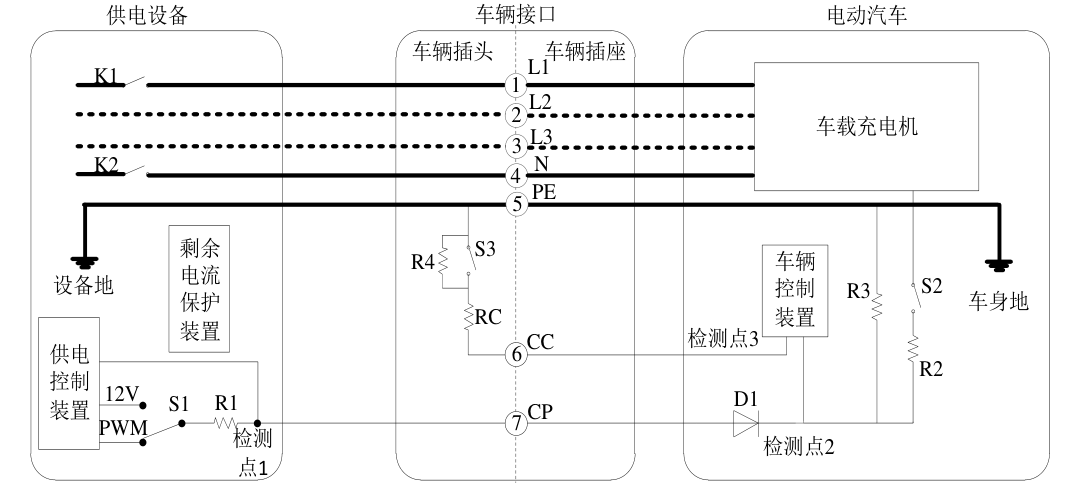
\includegraphics[width = 0.7\textwidth]{C2}
        \caption{车载充电机输入控制引导电路}
        \label{fig:C2}
    \end{figure}




\section{控制导引 (Control Pilot)}
	控制导引电路是确保在将电动汽车(EV)或插电式混合动力汽车(PHEV)连接到电动汽车供电设备(EVSE)时正确操作的主要控制手段。它包括安全有效充电所需的一系列事件和功能。

\subsection{控制导引电路参数和车辆状态}
	控制导引电路参数和车辆状态对于EV和EVSE之间的正确通信和控制至关重要。这些参数确保车辆状态(例如,已连接、准备充电)的正确识别和充电行为的正确执行。

\subsection{控制导引信号}
	控制导引信号用于通信EVSE和车辆的操作状态。具体的占空比由EV/PHEV解释为不同的操作命令:
	\begin{enumerate}
		\item 3-7\%的占空比:有效的数字通信命令。
		\item 8-10\%的占空比:解释为有效的10\%占空比。
		\item ≤85\%的占空比:根据电流(安培数) = 占空比(\%) * 0.6。
		\item 85\%的占空比:根据电流(安培数) = (占空比 - 64) * 2.5。
		\item 97\%的占空比:建议解释为有效的96\%占空比。
	\end{enumerate}

\subsection{控制导引容差}
控制导引信号的总体容差为±2\%,其中EVSE的容差为±0.5\%,EV/PHEV的容差可达±1.5\%。


\section{接近检测 (Proximity Detection)}

\subsection{接近检测电路} 
接近检测电路用于检测连接器插入车辆插口的情况,以防止在车辆移动时对连接器造成损坏。该检测涉及电阻器和连接到连接器锁扣释放执行器的机械开关。此检测可用于满足连接器断开电流限制和带有连接器耦合器的车辆移动的要求。

\subsection{接近检测电路参数 }
接近检测电路包括诸如电阻和开关等组件,确保检测到连接器的存在并提供必要的逻辑以确保安全和操作目的。对于交流(AC)充电,该电路的监测是可选的,但对于直流(DC)充电,该监测是强制性的。

接近检测电路参数具体要求如下:

+5V直流(调节):5.0V(标称值),最大值为5.25V,最小值为4.75V。
各种电阻(R4、R5、R6、R7)的等效负载电阻值,具有指定的标称值、最大值和最小值。
总结
控制导引和接近检测电路是确保EV和EVSE安全有效操作的重要部分。控制导引电路通过定义占空比来管理通信和充电状态,而接近检测电路通过检测连接器的存在来防止潜在的损坏和确保安全。两者都具有特定的参数和容差要求,以确保系统的可靠性和功能性。


